
% \begin{IB}
% comment exemple
% \end{IB}

%% \begin{TD} pour Tanguy et \begin{DG} pour Dom

%% ************************************************************

%% Context

%% *************************************************************
\section{Contexte}

La distribution de la vegetation est fortement déterminée par le climat.
Cependant, nombreuses sont les études montrant le déséquilibre entre la niche
fondamentale, c'est-à-dire l'espace écologique déterminé par les contraintes
physiologiques, et la niche réalisée, qui correspond à la projection des
observations d'occurrence (\textit{i.e}, dans l'espace géographique) dans
l'espace écologique. Parmi les différents facteurs qui peuvent expliquer cette
différence entre les deux niches, on trouve l'histoire biogéographique et la
capacité de dispersion des espèces, les perturbations (\textit{e.g.,} les
feux), ainsi que les interactions biotiques (intra et inter niveaux
trophiques).

\vspace{1em}

Ici on va s'intéresser plus largement aux transitions entre types de
végétation (écotones) et non pas à une espèce en particulier. Pour simplifier
le système, on ne considèrera pas l'espace de façon explicite et donc on ne
s'intéressera pas au rôle de la dispersion limitée. En plus d'inclure les
perturbations, notre étude se focalisera surtout sur le rôle potentiel des
grands herbivores, qui ont un impact avéré sur la régénération de la forêt.
D'autre part, la rétro-action de la végétation sur les populations
d'herbivores sera prise en compte. L'objectif sera d'évaluer l'importance de
ces interactions trophiques le long d'un gradient environnemental.

\vspace{1em}

Deux types d'écotones seront examinés: (1) La transition entre prairie et
forêt, et (2) La transition entre deux types de forêts.


%% ************************************************************

%% Questions

%% *************************************************************

\subsection*{Question générale}

Quelle est le rôle des grands herbivores sur les limites d'écosystèmes (écotones)?

\vspace{1em}

\begin{enumerate}

\item Le long d'un gradient environnemental au niveau de l'écotone, la
présence d'herbivores peut-elle décaler la transition (dans l'espace
écologique/géographique), modifier sa forme ?

\item Quel est l'impact des pesseurs et des brouteurs en interaction à
l'interface prairie/forêt ?

\item Quel est l'impact des pesseurs à l'interface forêt tempérée/boréale?

\end{enumerate}

%% ************************************************************

%% Abstract ESA

%% *************************************************************
\newpage

\section*{Abstract ESA}

\textbf{Background/Question/Methods}\\

Although it is widely recognized that ecological interactions are important to
maintain ecosystem properties, existing landscape level models usually account
for a small number of species and/or a single trophic level. In particular,
vegetation dynamic or distribution models rarely consider large herbivores as
key drivers, and even less they integrate feedback effects of the vegetation
on herbivores. However, it is possible geographical limits of some species or
ecosystems such as the treeline ecotones or the temperate-boreal forest
transition are the results of trophic interactions.

\vspace{1em}

Here we propose to examine how accounting for browsers and/or grazers in
interaction with the vegetation is likely to modify the vegetation equilibrium
states along an environmental gradient. We examine two cases: (1) How grazers
and/or browser might affect the treeline ecotones? (2) What role a browser
mainly feeding on the temperate trees might play in determining the ecotone
between temperate and boreal forests?

\vspace{1em}

We use simple mathematical models (differential equations) to represent the
transition between vegetation states. The herbivores' dynamics is modeled as a
biomass variation in time and uses a metaphysiological modelling approach.
Finally, trophic interactions between the vegetation and animal biomasses
include resources preferences depending on resource availability mediated by
climatic conditions.

\vspace{1em}

\textbf{Results/Conclusions}\\

Our preliminary simulations suggest that herbivores populations, through
complex trophic interactions, might be a significant factor limiting species
ranges and defining ecotones. This implies that in many places, the temperate
forest distribution might not be directly limited by physiological constraints
related to climatic conditions. In addition to fire, this could explain the
historical abundance of open environments in central Europe. In a context of
climate change, these results suggest that it is not possible to anticipate
the response of the vegetation whilst ignoring its interactions with other
trophic levels.


%% ************************************************************

%% FIRST MODEL

%% *************************************************************
\newpage
\section{Vegetation model}

Three vegetation states $G$, $S$, and $T$ describe respectively the
proportions of Grasslands, Seedling-dominated, and Forest habitats.

\vspace{2em}

\begin{center}
\vspace{5em}
\tikz[baseline]{\node[draw, circle, anchor=base] (G){G};} \hspace{5em}
\tikz[baseline]{\node[draw, circle, anchor=base] (S){S};} \hspace{5em}
\tikz[baseline]{\node[draw, circle, anchor=base] (T){T};} 
\end{center}

\begin{tikzpicture}[overlay]
\draw[-angle 45] (G.east) -- (S.west) node[midway,below] {$cfT$};
\draw[-angle 45] (S.east) -- (T.west) node[midway,below] {$\alpha$};
\draw[-angle 45] (T.north) to[bend right=50] node[midway,above] {$\delta(1-cfT)$} (G.north) ;
\draw[-angle 45] (T.north) to[bend right=50] node[near end,above] {$\delta cfT$} (S.north) ;
\end{tikzpicture}

\vspace{1em}

%-----
\[
\left\{
\begin{array}{r c l}

G &=& 1 - T - S\\

\rule{0pt}{7ex} \frac{dT}{dt} &=& 
\overbrace{\alpha S}^\text{succession} - \overbrace{\delta T}^\text{disturbances}\\

\rule{0pt}{7ex} \frac{dS}{dt} &=& 
\overbrace{fT}^\text{seeds}
\overbrace{c(G+\delta T)}^\text{colonisation}
-
\overbrace{\alpha S}^\text{succession} \\

\end{array}
\right.
\]

\vspace{1em}

$\alpha$ is the succession rate (inverse of maturity age)

$\delta$ is the disturbance rate (includes fire and other events)

$c$ is the competitive success of seedlings on grasses

$f$ is the trees' fecundity (i.e., seedling production)


This system has one stable state:

\[
\left\{
\renewcommand{\arraystretch}{2}
\begin{array}{r c l}{}

G^\ast &=& \frac{\delta(\alpha cf-\alpha-\delta)}{cf(\alpha \delta-\alpha-\delta)}\\

T^\ast &=& \frac{\alpha(\delta-cf)}{cf(\alpha \delta-\alpha-\delta)}\\

S^\ast &=& \frac{\delta(\delta-cf)}{cf(\alpha \delta-\alpha-\delta)}\\

\end{array}
\right.
\]

Note that $\frac{S^\ast}{T^\ast} = \frac{\delta}{\alpha}$, the equilibrium
depends on the disturbance rate to succession rate ratio.

%----------
\newpage
\subsection*{Equilibrium along the gradient}

All parameters may respond in their way to the climate. However, the main
response of the vegetation, the most documented, is related to the
recruitment. Therefore $c$ should be a function of the environment. A high $c$
allows the forest to dominate whilst a lower $c$ is favourable to grasslands.
\\

If this function is linear, the vegetation equilibrium along a gradient of
this parameter is illustrated below for three different values of $\delta$

\begin{figure}[!h]
   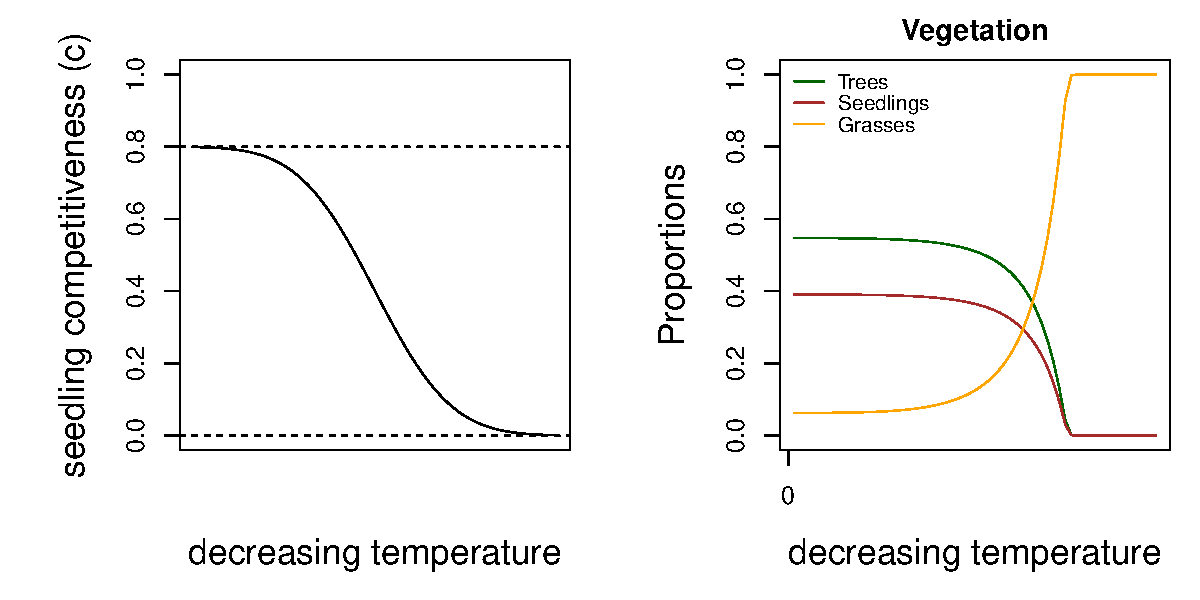
\includegraphics[width=0.9\textwidth]{../graphs/Mod1_climate.pdf}

   \caption{Equilibrium has been computed along a gradient of $c$ (success of
seedlings on grasses for establishment). $\alpha$ = 0.07; f = 1; $\delta$
varies among 0.03 (dashed); 0.05 (solid) and 0.07 (dotted)}
\label{mod1Climate} 
\end{figure}



%% ************************************************************

%% Incorporating two tree species

%% *************************************************************
\newpage
\section{Model with two forest types}

In this case the forest is divided into two types $C$ and $D$ for conifer and
deciduous dominated ecosystem (\textit{e.g.} boreal vs temperate forest). The
seedling state do not distinguished between the two potential future forest
types. It is considered as a transition state.

\vspace{2em}
\begin{center}
\begin{tikzpicture}
\matrix(m) [matrix of nodes, column sep=6em,
	row sep=2em,
	minimum width=1em,
	minimum height=1em,
	nodes={draw, circle, anchor=base}]
	{
	& & C \\
	G & S & \\
	& & D \\
	}; %end matrix

\draw[-angle 45] (m-2-1.east) -- (m-2-2.west) node[midway,below] {$cf_{C}C + cf_{D}D$};
\draw[-angle 45] (m-2-2.north east) -- (m-1-3.west) node[midway,above] {$\alpha_C k$};
\draw[-angle 45] (m-2-2.south east) -- (m-3-3.west) node[midway,above] {$\alpha_D (1-k)$};
\draw[-angle 45] (m-1-3.north west) to[bend right=50] node[midway,above] {$\delta_C cf_{C}C$} (m-2-2.north) ;
\draw[-angle 45] (m-3-3.south west) to[bend left=50] node[midway,below] {$\delta_D cf_{D}D$} (m-2-2.south) ;
\draw[-angle 45] (m-1-3.north) to[bend right=50] node[midway,above] {$\delta (1-cf_{C}C)$} (m-2-1.north) ;
\draw[-angle 45] (m-3-3.south) to[bend left=50] node[midway,below] {$\delta (1-cf_{D}D)$} (m-2-1.south) ;

\end{tikzpicture}
\end{center}

\vspace{1em}

%-----
\[
\left\{
\begin{array}{r c l}

G &=& 1 - C - D - S\\

\rule{0pt}{7ex} \frac{dC}{dt} &=& 
\overbrace{\alpha_C kS}^\text{succession} - \overbrace{\delta_C C}^\text{disturbances}\\

\rule{0pt}{7ex} \frac{dD}{dt} &=& 
\overbrace{\alpha_D (1-k)S}^\text{succession} - \overbrace{\delta_D D}^\text{disturbances}\\

\rule{0pt}{7ex} \frac{dS}{dt} &=& 
c(
\overbrace{G(f_C C + f_D D)}^\text{colonisation of G}
+
\overbrace{\delta_C f_C C + \delta_D f_D D}^\text{colonisation of disturbed forests}
)
-
\overbrace{(\alpha_C k + \alpha_D (1-k)) S}^\text{succession} \\

\end{array}
\right.
\]

\vspace{1em}

$\alpha_C$ and $\alpha_D$ are the succession rates (inverse of maturity age)

$\delta_C$ and $\delta_D$ are the disturbance rates

$c$ is the competitive success of seedlings on grasses

$f_C$ and $f_D$ are the fecundities (i.e., seedling production)

$k$ is the competitive success of conifers on deciduous seedlings

\vspace{1em}

N.B.1 Only a browser would be considered and only affect $D$\\

N.B.2 This is a similar case to the one I would explore with a spatially
explicit, cohort-based model of trees' dynamics and its interaction with an
herbivore (browser) population.

%----------
\newpage
\subsection*{Equilibrium along the gradient}

Here, the main response of the vegetation, the one important to determine the
gradient, related to the recruitment, is related to $k$ (competitiveness of
conifers on deciduous). A high $k$ allows the (boreal) forest to dominate
whilst a lower $k$ is favourable to the temperate trees. \\ The vegetation
equilibrium along a gradient of this parameter is illustrated below.

\begin{figure}[!h]

   \includegraphics[width=\textwidth]{../graphs/env_gradient2.pdf}

\end{figure}

\begin{SCfigure}[1][h]

   \includegraphics[width=0.6\textwidth]{../graphs/Mod2_climate.pdf}

   \caption{Equilibrium has been computed along a gradient of $k$ (success of
conifers seedlings on deciduous seedlings). $\alpha_C$ = $\alpha_D$ = 0.07;
$f_C$ = $f_D$ = 1; $\delta_C$ = $\delta_D$ = 0.05; $c$ =0.05}
\label{mod2Climate} 
\end{SCfigure}



%% ************************************************************

%% Herbivore 

%% *************************************************************
\newpage
\section{Herbivores' dynamics}

Based on metaphysiological model \cite{Owen-Smith2002}

The herbivore dynamic will be modelled as a total biomass in the considered
landscape (AND NOT a number!)

%-----
\[
\left.
\begin{array}{r c l}{}

\frac{dH}{dt} &=& 
\overbrace{H*I}^\text{biomass gains} - \overbrace{H*(p+qe^{-zI}+m)}^\text{biomass losses})

\end{array}
\right.
\]

%-----

\vspace{1em}

$p$ is the metabolic attrition rate (per herbivore biomass unit)

$q$ is the maximum mortality rate due to starvation (per herbivore biomass unit)

$z$ is a decreasing parameter of mortality rate in function of intake

$m$ is the minimum mortality rate when food is abundant (senescence, accidents, hunting...)

$I$ is the vegetation intake rate (consummed biomass per herbivore biomass unit - see next section for details)

\vspace{1em}

Gains=losses=$I_K$ when:

\[
I_K = m + p + \frac{1}{z}LambertW(qze^{-z(m+p)})
\]


\begin{SCfigure}[0.9][h]
\centering
   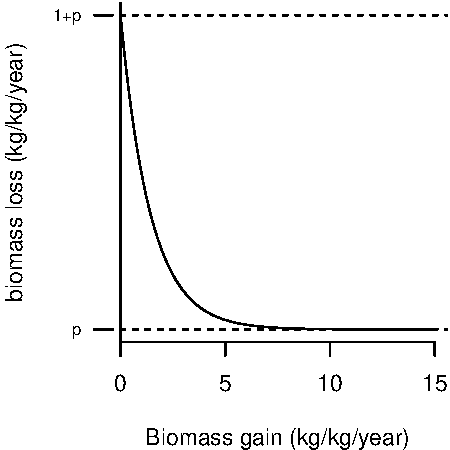
\includegraphics[width=0.5\textwidth]{../graphs/herbivore_mortality.pdf}

   \caption{Herbivore mortality depends on the intake. The figure illustrates
   this relationship for p = 0.1; q = 0.7; z = 0.2; m = 0.1}

\label{herbiMort} 
\end{SCfigure}


\newpage
%% ************************************************************

%% resources intakes 

%% *************************************************************
\section{Effect of the vegetation on herbivores: resources intakes}

The intake (biomass consumption per herbivore biomass per time unit) will
depend on available resource and the herbivore preferences to have the best
quality food. Let's $R_1$ be the available preferred resource and $R_2$ the
available secondary resource (per herbivore biomass unit). The intake from
$R_2$ will depend on the relationship between the intake from $R_1$ and $p+m$
(minimum biomass loss rate).

\[
I = \overbrace{\frac{\tau R_1}{\mu+R_1}}^\text{intake rate of preferred resource} 
+ \overbrace{\frac{\theta R_2}{\nu+R_2}\frac{1}{1+e^{r(\frac{\tau R_1}{\mu+R_1} - p - m)}}}^\text{intake rate of secondary resource} 
\]

$\tau$ and $\theta$ are the maximum rates of intake (vegetation biomass per
herbivore biomass) including digestibility... CAN BE >1. Should be >$I_K$ for
allowing herbivore positive growth.

$\mu$ and $\nu$ are a half saturation parameter for resource intake (available
resource for which the intake is half)

$r$ is a smoothing parameter for the swich between use/non-use of the non-
preferred resource


\begin{SCfigure}[1][h]
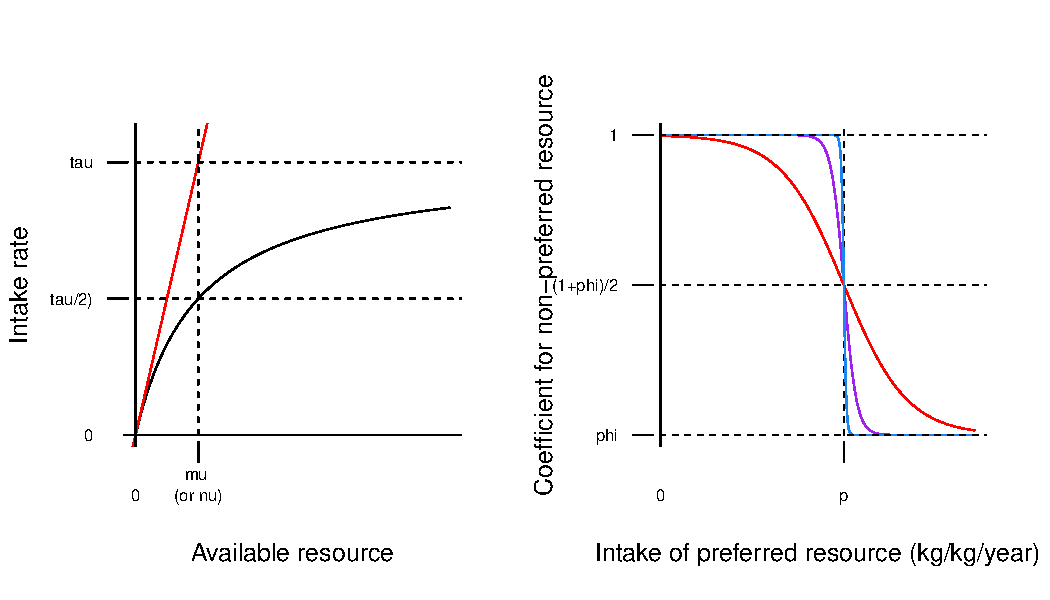
\includegraphics[width=0.7\textwidth]{../graphs/intakes.pdf}
   
   \caption{Use of resources. The figure illustrates the mechanisms for p = 0.1; q = 0.7; z = 0.2; m = 0.1; $\tau$ = 5; $\mu$ = 20; r = 20}
\label{resources}
\end{SCfigure}

Preferred resources $R_1 = kuS/H_b$ for $H_b$ and $R_1 = wG/H_g$ for $H_g$, and non-preferred resource $R_2=vT/H_b$ for $H_b$ and $R_2= (1-k)uS/H_g$ for $H_g$).\\

$u$, $v$, and $w$ are conversions between areas and available biomass (i.e., vegetation density, accessibility), and $k$ is the competitive ability of browser on grazer to consum $S$.

\[
k = e^{-k_0\frac{H_g}{H_b}}
\]

In order to match these conditions:
\[
\left.
\begin{array}{l}
k = 1 \text{ if } H_g=0\\
k = 0 \text{ if } H_b=0\\
k = k_0 \text{ if } H_b=H_g
\end{array}
\right.
\]


\paragraph{Range of variation}

$I_b \in$ [0; max($\tau_b k; \theta_b$)]
et
$I_g \in$ [0; max($\tau_g, \theta_g (1-k)$)]

\newpage
\subsection*{Existence and coexistence conditions}

There is a positive growth rate if $I>I_K$\\

These conditons are fullfilled when:\\

(for the browser) 
$$\iff T = H_b \frac{-f(S, H_b)\nu_b}{v(f(S, H_b)-theta_b)}$$ 
with $$f(S, H_b) = (1+e^{r_b(\frac{\tau_b kuS/H_b}{\mu_b+kuS/H_b} - p_b - m_b)} ) (I_Kb - \frac{\tau_b kuS/H_b}{\mu_b + kuS/H_b})$$

(for the grazer) 
$$\iff S = H_g \frac{-f(G, Hg)\nu_g}{(1-k)u(f(G, H_g)-theta_g)}$$
with $$f(G, H_g) = (1+e^{r_g(\frac{\tau_g wG/H_g}{\mu_g+wG/H_g} - p_g - m_g)} ) (I_Kg - \frac{\tau_g wG/H_g}{\mu_g + wG/H_g})$$

\begin{figure}[h]
\centering
\includegraphics[width=0.4\textwidth]{../graphs/existenceHb.pdf}
\includegraphics[width=0.4\textwidth]{../graphs/existenceHg.pdf}
  \caption{Conditions of existence of the two types of herbivore separately. The black solid line indicates the intake at which gains equals losses for the herbivore population. In this exemple the parameters are u = 6000; v=3000; w=5000; $\tau_b$ = $\tau_g$ = 6; $\theta_b$ = $\theta_g$ =5; $\mu_b = \mu_g = \nu_b = \nu_g$ =30; $r_b = r_g$ = 20; $p_b = p_g = m_b = m_g$ = 0.05; $q_b = q_g$ = 0.8; $z_b = z_g$ = 10}
\label{existenceH}
\end{figure}

\newpage 
For each landscape proportions, we are able to estimate the two
coexisting herbivore biomasses at equilibrium solving

\[
\left\{
\begin{array}{r c l}
Ik_b &=& I_b \\
Ik_g &=& I_g
\end{array}
\right.
\]
We know that intakes depend on $H_g$, $H_b$, S, T, and G
\[
\left\{
\begin{array}{r c l}
Ik_b &=& I_b = f(H_g, H_b, S, T) \\
Ik_g &=& I_g = f(H_g, H_b, S, G)
\end{array}
\right.
\]

Which means that $H_b$ can be expressed depending on these variables in two
different ways (not analytically, I am not able neither the computer).

\[
\left\{
\begin{array}{r c l}
H_b &=& f(H_g, S, T) \\
H_b &=& f(H_g, S, G)
\end{array}
\right.
\]

We are thus able to find numerically the amount of $H_b$ and $H_g$ at
equilibrium for each {G,S,T} combinations. Sometimes, there is no possible
coexitence. \\

With the same parameters as before, we get:

\begin{SCfigure}[1][h]
\includegraphics[width=0.7\textwidth]{../graphs/coexistence_herbivores.pdf}
  \caption{Conditions of co-existence of the two types of herbivore. In this exemple the parameters are $k_0$ =0.6; u = 6000; v=3000; w=5000; $\tau_b$ = $\tau_g$ = 6; $\theta_b$ = $\theta_g$ =5; $\mu_b = \mu_g = \nu_b = \nu_g$ =30; $r_b = r_g$ = 20; $p_b = p_g = m_b = m_g$ = 0.05; $q_b = q_g$ = 0.8; $z_b = z_g$ = 10}
\label{coexistenceH}
\end{SCfigure}

\newpage
%% ************************************************************

%% feedbacks on vegetation 

%% *************************************************************
\section{Feedback effects: impacts on the vegetation}

Based on the fact that the impact on demography is as much or more important
than the impact on biomass (\cite{Moncrieff2014}).

The herbivores will affect $c$ depending on the herbivore pressure on $G$
($P_G$) and on $S$ ($P_S$) and will affect $\alpha$ depending on the pressure
on $S$ ($P_S$). \\ $c$ is expected to decrease from $c_0$ to 0 proportional to
$U_S$ when $U_G=0$ and to increase from $c_0$ to 1 proportional to $P_G$ when
$P_S=0$:

\[
c = f(S, G) = P_G - c_0(P_G+P_S) + c_0
\]

$\alpha$ decreases from $\alpha_0$ to 0 proportional to $P_S$:

\[
\alpha = f(S, G) = \alpha_0(1-P_S)
\]

\begin{figure}[h]
\begin{center}
\includegraphics[width=\textwidth]{../graphs/effectsOnVeg.pdf}
\caption{Illustration of the variation of $c$ and $\alpha$ according to the herbivore pressure}
\end{center}
\end{figure}

\subsection*{Forest-grasslands ecotone}

Let's $U_S$ be the total intake of $S$, $U_{b1}$ the intake from the browser on $S$ and $U_{g2}$ the intake from the grazer on $S$.

\[
U_S = \overbrace{H_b\frac{\tau_b kuS/H_b}{\mu_b+kuS/H_b}}^\text{$I_{b1}$} 
+ \overbrace{H_g\frac{\theta_g (1-k)uS/H_g}{\nu_g+(1-k)uS/H_g}\frac{1}{1+e^{r_g(\frac{\tau_g wG/H_g}{\mu_g+wG/H_g} - p_g - m_g)}}}^\text{$I_{g2}$}
\]

$P_S = \frac{U_S}{uS}$ is the pressure on S (proportion of total intake among available food) varying from 0 to 1.

\[
P_S = f(S, G, H_b, H_g) = \frac{\tau_b k}{\mu_b+kuS/H_b}
 + \frac{\theta_g (1-k)}{\nu_g+(1-k)uS/H_g}\frac{1}{1+e^{r_g(\frac{\tau_g wG}{\mu_g*H_g+wG} - p_g - m_g)}}
\]

Similarly $P_G$ the pressure on $G$ depends on $U_{g1}$ the intake of the grazer on $G$:

\[
P_G = f(G, H_g) =\frac{U_{g1}}{wG} = \frac{\tau_g}{\mu_g+wG/H_g}
\]


% REVOIR !!!
\subsection*{Forest-forest ecotone}

In this case, there is only $P_S$ which is

\[
P_S = f(S, D, H_b) =\frac{\tau_b k}{\mu_b+uS/H_b}
\]
% REVOIR !!!


%% ************************************************************

%% Effects of herbivores: illustration

%% *************************************************************

\newpage
\subsection*{Effects of a constant herbivore pressure on the vegetation}

\subsubsection*{Browsers and grazers in a forest-grassland ecotone}

\begin{figure}[!h]
\includegraphics[width=.9\textwidth]{../graphs/Mod1_herbivore2.pdf}
\caption{Illustration of the variation of vegetation proportion at equilibrium according to the herbivores abundances. Parameters are the same as before.}
\end{figure}

\newpage
\subsubsection*{Browser in a forest-forest ecotone}

\begin{figure}[!h]
\includegraphics[width=.9\textwidth]{../graphs/Mod2_herbivore.pdf}
\caption{Illustration of the variation of vegetation proportion at equilibrium according to the herbivores abundances. Parameters are the same as earlier.}
\end{figure}


%% ************************************************************

%% couplage

%% *************************************************************
\newpage
\section{Coupling both models}
\subsection*{Forest-grassland ecotone}

\begin{figure}[!h]
\centering
\includegraphics[width=.8\textwidth]{../graphs/Mod1H_combinated_veg.pdf}
\includegraphics[width=.8\textwidth]{../graphs/Mod1H_combinated_herb.pdf}
\caption{Illustration of the variation of vegetation proportion at equilibrium and herbivores abundances when interactions are considered in the two ways simultaneously. Parameters are the same as earlier.}
\end{figure}

\newpage
\subsection*{Forest-forest ecotone}

\begin{figure}[!h]
\centering
\includegraphics[width=.8\textwidth]{../graphs/Mod2H_combinated.pdf}
\caption{Illustration of the variation of vegetation proportion at equilibrium and herbivores abundances when interactions are considered in the two ways simultaneously. Parameters are the same as earlier.}
\end{figure}


%% ************************************************************

%% Along the gradient 

%% *************************************************************
\newpage
\section{Effects of the environment in the combined models}

In addition to affecting $c$ (i.e., recruitment) and $k$ (conifer/deciduous
seedling competitiveness), the environment will directly affect the vegetation
through its available biomasses for the herbivores ($u$, $v$, $w$).

$u$, $v$, and $w$ might be affected by precipitations (biomass production)

\vspace{1em}
\begin{IB}
$w$ might also be affected by the quantity of snow (grasses accessibility)

$\delta$ (disturbances on trees) might be affected by winds (frequency of storms)

Herbivores might be directly affected by extreme temperature (in a second
analyse maybe) but the impact will be mostly mediated by the vegetation
response.\\ 
ex. mooses do not tolerate warm temperature -> use forest as
refuges (Melin 2013)
\end{IB}

\subsection*{Parameter variation along an environmental gradient}

\begin{figure}[!h]
\centering
\includegraphics[width=.5\textwidth]{../illustrations/biomes3bis.pdf}
\includegraphics[width=.4\textwidth]{../graphs/environmental_gradient.pdf}
\caption{Biomes and climate (left)}
\caption{Effect of the environment on parameters (right)}
\end{figure}

From temperate to boreal forest (taiga), precipitation and temperature simultaneously decrease. At the tree line in the Alps or in the Artic, the change is similar (precipitation and temperature decrease).

The environmental gradient will therefore illustrate both tendencies. $c$ will decrease, as well as $u$, $v$ and $w$. $k$ will increase.


\newpage
\subsection*{Analysis along the gradient}

\begin{figure}[!h]
\centering
\includegraphics[width=\textwidth]{../graphs/Mod1H_combinated_env.pdf}
\caption{Effect of herbivores and on their feedback on the vegetation, along an environmental gradient}
\end{figure}

\newpage
\begin{figure}[!h]
\centering
\includegraphics[width=\textwidth]{../graphs/Mod2H_combinated_env.pdf}
\caption{Effect of herbivores and on their feedback on the vegetation, along an environmental gradient}
\end{figure}



%% ************************************************************

%% Parameters 

%% *************************************************************
\newpage
\section{Parameters values (for discussion and corrections and planning sensibility analysis)}

%---------------------------------
\subsection*{Vegetation models}

$\alpha$ (succession rate) = 0.07 which corresponds to a mature age of 14

\noindent $\delta$ (disturbance rate) = 0.05 which corresponds to intensity * frequency = 0.75 * 1/25

\noindent $f$ (fecundity) = 1 which means that one tree portion is capable to colonize maximum one free portion of the landscape

\noindent I did not put any difference between temperate and boreal trees for these params.

\noindent $c$ (seedlings competitiveness over grasses) = 0.8 which means that they outcompete grasses. But this varies according to the environment (see below)

\noindent $k$ (Conifers competitiveness over deciduous) = 0.5 for exemples and varies according to the environment (see below)


%---------------------------------
\subsection*{Herbivore model}

$\tau$ (saturation of intake rate) = 6 which means that an animal could not consum more than 6 times its own biomass of the preferred resource

\noindent $\theta$ =5 which means the same thing for the secondary resource

\noindent $\mu$ (half saturation parameter) = 30 which means that when available biomass is 30 (kg) the intake rate is equals to half its maximum

\noindent $\nu$ = 30 : same thing for the secondary resource

\noindent $p$ (metabolic attrition rate) = 0.05 which means that 5\% of biomass is lost by metabolic attrition

\noindent $m$ (minimum mortality rate when resource is abundant) = 0.05 which means 5\% of biomass (or animals) are lost due to other factors 

\noindent $q$ (maximum mortality rate due to starvation) = 0.8 which means that 20\% of animals biomass 'survives' if there is no resource

\noindent $z$ (exponential decrease of mortality when intake increases) = 10 which means that biomass loss reduces 10 times more than exponential minus intake

\noindent $r$ (smoothing parameter for switch to use the secondary resource) = 20 I guess it has few importance. Maybe test its sensitivity?

\noindent I did not put any difference between browsers and grazers for these params.


\noindent $k_0$ (competitiveness of browser over grazer for seedling resource when they have equal abundance) = 0.8 which mean that 80\% of available seedlings is actually available for the browser and 20\% for the grazer in this case.

%---------------------------------
\subsection*{Interactions}

\noindent $u$ (available biomass from seedlings) = 6000 which mean that the landscape considered would provide 6000 (kg) of digestible and accessible resource for herbivores if it were entirely covered by seedlings.

\noindent $v$ = 3000 idem for trees (or temperate trees)

\noindent $w$ =5000 idem for grasses biomass 

%---------------------------------
\subsection*{Environmental gradient}

$c$ (seedlings competitiveness over grasses) varies logistically from 0.8 to 0 (forest-grasslands) and from 0.8 to 0.2 (temperate-boreal).

\noindent $k$ (conifers competitiveness over deciduous) varies from 0 to 1 (temperate-boreal)

\noindent $u$, $v$, $w$ (vegetation biomasses) are multiplied by a factor that varies from 1 to 0.2

